\section{Auswertung}
\label{sec:Auswertung}

% \begin{figure}
%   \centering
%   \includegraphics{plots/plot.pdf}
%   \caption{Plot.}
%   \label{fig:plot}
% \end{figure}



% \begin{table}
%    % Notation :  {% nicht entfernen ist sehr wichtig sonst Fehler !!
% \parbox{0.48\textwidth}{% %Ermöglicht zwei Tabellen neben einander
%   \centering
%   \sisetup{round-mode = places , round-precision = 0,scientific-notation=fixed, fixed-exponent = 0}
%          %rundet Werte aus Stelle, Stelle = ,  macht einen bestimmten festen exponenten
%   \resizebox{\textwidth}{!}{%  % skaliert zu große Tabellen
%   \begin{tabular}{S@{${}\pm{}$} S} % fügt plus minus Fehler Schreibweise hinzu
%     \toprule
%      $\text{e}_b / \si{\milli\meter}$ &
%      $\text{d}_b /\si{\milli\meter} $ & $\text{f}_b / \si{\milli\meter} $\\
%     \midrule
%     \bottomrule
%   \end{tabular}
%   % }
%   \caption{Tabellenunterschrift}
%   \label{tab:tab}
% }
% % \end{table}
% % \begin{table}
% \parbox{0.48\textwidth}{%
%   \centering
%   \sisetup{round-mode = places , round-precision = 0,scientific-notation=fixed, fixed-exponent = 0}
%   % \resizebox{\textwidth}{!}{%
%   \begin{tabular}{S@{${}\pm{}$} S}
%     \toprule
%      $\text{e}_b / \si{\milli\meter}$ &
%      $\text{d}_b /\si{\milli\meter} $ & $\text{f}_b / \si{\milli\meter} $\\
%     \midrule
%     \bottomrule
%   \end{tabular}
%   % }
%   \caption{Tabellenunterschrift}
%   \label{tab:tab}
% }
% \end{table}
\subsection{Hysterese Kurve des Magnetfeldes}
Die Feldstärke $B$ wird gegen den Feldstrom $I$, in Abbildung \ref{fig:BFeldplot}, aufgetragen. 
Das ermöglicht später das Magnetfeld zu berechnen, bei dem die Aufspaltung der Spektrallinien 
zu beobachten ist. In der Abbildung wird durch den linearen Teil der aufsteigenden Hysteresekurve eine 
Ausgleichsgerade gelegt. Die abfallende Hysteresekurve wurde zur Vollständigkeit gemessen und 
eingetragen. Die Ausgleichsrechnung wird mit Hilfe von \cite{scipy} und der Funktion
\begin{equation*}
B\left(I\right) = a \cdot I + b
\end{equation*}
durchgeführt.  Daraus ergibt sich $ a = \SI{61.7(4)}{\milli\tesla\per\ampere}$ und 
$ b = \SI{9(3)}{\milli\tesla}$. Die in Abbildung \ref{fig:BFeldplot} schwarz markierten Werte wurden 
in der Ausgleichsrechnung nicht betrachtet, da diese nicht mehr im linearen Teil der Hysteresekurve 
liegen.
\begin{figure}
  \centering
  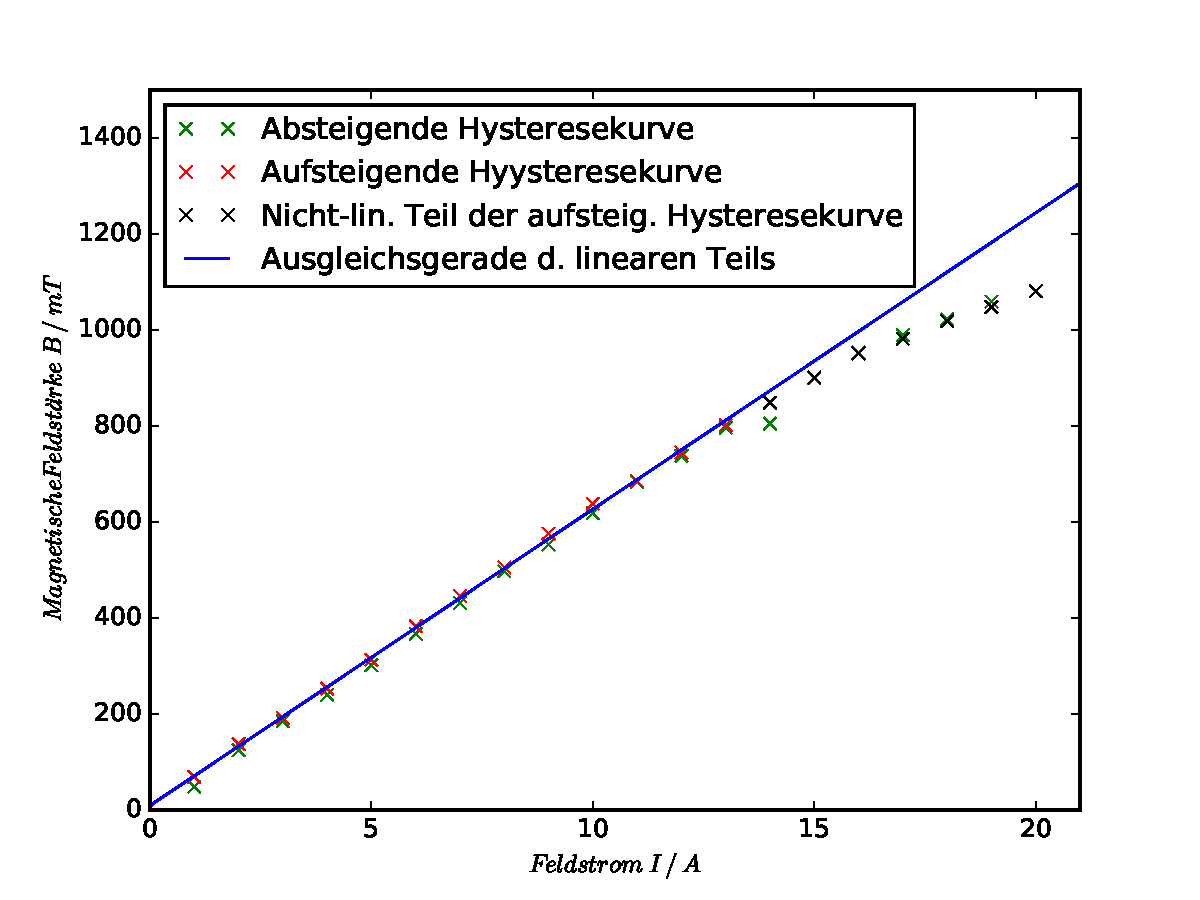
\includegraphics[height = 7cm]{plots/BFeldplot.pdf}
  \caption{Auf- und absteigende Hysterese Kurve des Magnetfeldes mit Ausgleichsgerade für den linearen Teil.}
   \label{fig:BFeldplot}
\end{figure}


\subsection{Methode zur Auswertung des Bildmaterials}
Das Bildmaterial wurde zuerst mit \textit{Fiji} \cite{fiji} ausgewertet, indem ein Intensitätsplot 
erstellt wurde, diese sind in den Abbildungen \ref{fig:p1},\ref{fig:p2}, \ref{fig:p3}, 
\ref{fig:p4}, \ref{fig:p5} und \ref{fig:p6} zu betrachten. Anschließend wurde aus den Plots die 
Position der Intensitätsmaxima ausgelesen. Der Abstand zwischen diesen Maxima wird dann $\Delta s$ 
oder $\delta s$ bei Aufspaltung eines Maximums bezeichnet.

\subsection{Zeeman-Effekt beim Übergang von \texorpdfstring{${}^1\symup{P}_1 \iff {}^1 \symup{D}_2$}{math} in Cadmium}

\begin{figure}
\centering
\caption{Spektrallinie des \texorpdfstring{${}^1\symup{P}_1 \iff {}^1 \symup{D}_2$}{math} Übergangs.}
\begin{subfigure}{0.48\textwidth}
  \centering
  
\includegraphics[height=5cm]{pics/644nm_B=0_P=0.JPG}
  \caption{Ohne Magnetfeld.}
  \label{fig:roto}
\end{subfigure}
\begin{subfigure}{0.48\textwidth}
  \centering
  
\includegraphics[height=5cm]{pics/644nm_I=9.5A_P=0.JPG}
  \caption{Mit Magnetfeld \texorpdfstring{$B = \SI{596(2)}{\milli\tesla}$}{math}.}
  \label{fig:rotb}
\end{subfigure}
\label{fig:rot}
\end{figure}


\begin{figure}
  \centering
  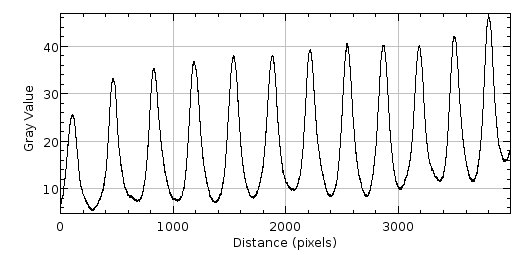
\includegraphics[height=5cm]{pics/Plot_644nm_B=0_P=0.jpg}
  \caption{Plot.}
  \label{fig:p1}
\end{figure}

\begin{figure}
  \centering
  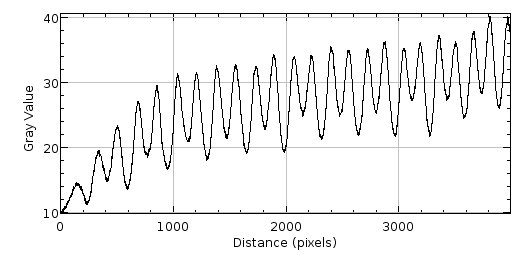
\includegraphics[height=5cm]{pics/Plot_644nm_I=9.5A_P=0.jpg}
  \caption{Plot.}
  \label{fig:p2}
\end{figure}

\begin{table}
\parbox{0.48\textwidth}{% 
  \centering
  \sisetup{round-mode = places , round-precision = 0,scientific-notation=fixed, fixed-exponent = 0}
  \begin{tabular}{S} 
    \toprule
    $\text{Position der Intensitätsmaxima} / \symup{px} $\\
    \midrule
      1.090000000000000000e+02\\
      4.680000000000000000e+02\\
      8.310000000000000000e+02\\
      1.186000000000000000e+03\\
      1.536000000000000000e+03\\
      1.883000000000000000e+03\\
      2.217000000000000000e+03\\
      2.542000000000000000e+03\\
      2.868000000000000000e+03\\
      3.185000000000000000e+03\\
      3.494000000000000000e+03\\
      3.803000000000000000e+03\\
    \bottomrule
  \end{tabular}
  \caption{Tabellenunterschrift}
  \label{tab:tab}
}
\parbox{0.48\textwidth}{%
  \centering
  \sisetup{round-mode = places , round-precision = 0,scientific-notation=fixed, fixed-exponent = 0}
  \begin{tabular}{S}
    \toprule
     $\text{Gangunterschied}\; \Delta s / \symup{px} $\\
    \midrule
      3.590000000000000000e+02\\
      3.630000000000000000e+02\\
      3.550000000000000000e+02\\
      3.500000000000000000e+02\\
      3.470000000000000000e+02\\
      3.340000000000000000e+02\\
      3.250000000000000000e+02\\
      3.260000000000000000e+02\\
      3.170000000000000000e+02\\
      3.090000000000000000e+02\\
      3.090000000000000000e+02\\
    \bottomrule
  \end{tabular}
  \caption{Tabellenunterschrift}
  \label{tab:tab}
}
\end{table}

\begin{table}
  \centering
  \sisetup{round-mode = places , round-precision = 0,scientific-notation=fixed, fixed-exponent = 0}
  \begin{tabular}{S S S}
    \toprule
     \multicolumn{2}{c}{$\text{Postion der Aufspaltungsmaxima} /\symup{px} $} 
     & $\text{Aufspaltung}\; \delta s /\symup{px}  $\\
    \midrule
      3.380000000000000000e+02 & 5.080000000000000000e+02 & 1.700000000000000000e+02\\
      6.920000000000000000e+02 & 8.560000000000000000e+02 & 1.640000000000000000e+02\\
      1.041000000000000000e+03 & 1.207000000000000000e+03 & 1.660000000000000000e+02\\
      1.387000000000000000e+03 & 1.556000000000000000e+03 & 1.690000000000000000e+02\\
      1.737000000000000000e+03 & 1.891000000000000000e+03 & 1.540000000000000000e+02\\
      2.073000000000000000e+03 & 2.225000000000000000e+03 & 1.520000000000000000e+02\\
      2.391000000000000000e+03 & 2.556000000000000000e+03 & 1.650000000000000000e+02\\
      2.722000000000000000e+03 & 2.879000000000000000e+03 & 1.570000000000000000e+02\\
      3.046000000000000000e+03 & 3.190000000000000000e+03 & 1.440000000000000000e+02\\
      3.346000000000000000e+03 & 3.506000000000000000e+03 & 1.600000000000000000e+02\\
      3.670000000000000000e+03 & 3.811000000000000000e+03 & 1.410000000000000000e+02\\
    \bottomrule
  \end{tabular}
  \caption{Tabellenunterschrift}
  \label{tab:tab}
\end{table}


\FloatBarrier




\subsection{Zeeman-Effekt beim Übergang von \texorpdfstring{${}^3\symup{S}_1 \iff {}^3 \symup{P}_2$}{math} in Cadmium}

\paragraph{\texorpdfstring{$\sigma$}{math}-Polarisation}




\begin{figure}[h!]
 \centering 
 \begin{subfigure}{0.48\textwidth}
  \centering
  
\includegraphics[height=5cm]{pics/480nm_B=0_P=0.JPG}
  \caption{Plot.}
  \label{fig:plot}
 \end{subfigure}
 \begin{subfigure}{0.48\textwidth}
  \centering
  
\includegraphics[height=5cm]{pics/480nm_I=5.5_P=0.JPG}
  \caption{Plot.}
  \label{fig:plot}
 \end{subfigure}
\end{figure}

\begin{figure}[h!]
  \centering
  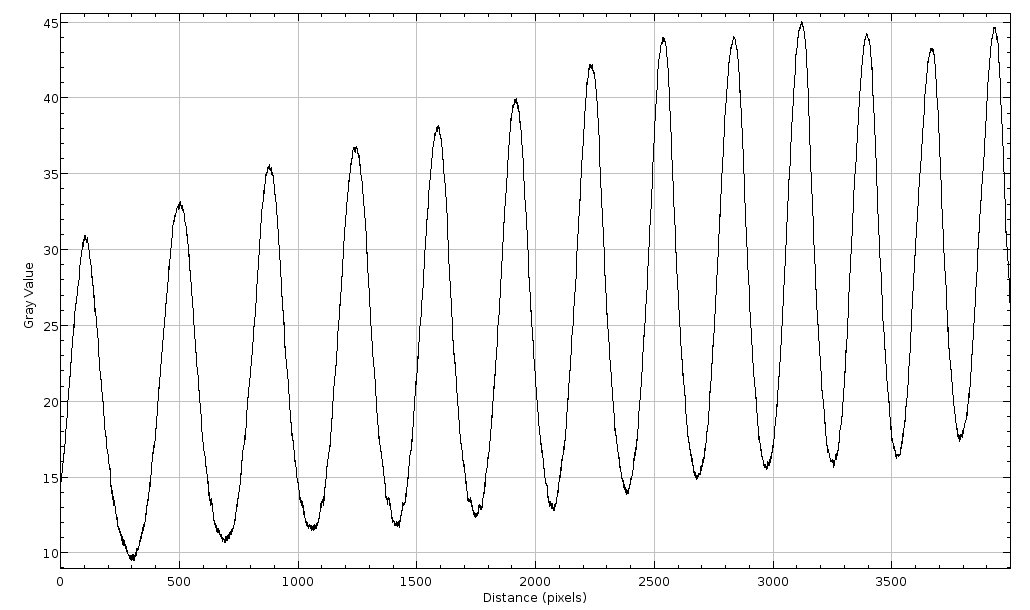
\includegraphics[height=5cm]{pics/Plot_480nm_B=0_P=0.jpg}
  \caption{Plot.}
  \label{fig:p3}
\end{figure}
\begin{figure}[h!]
  \centering
  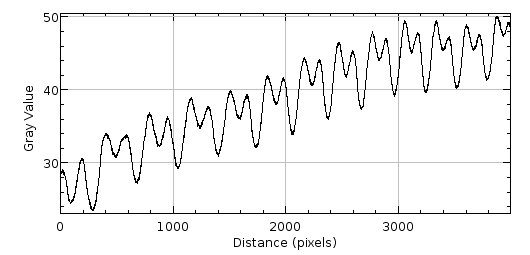
\includegraphics[height=5cm]{pics/Plot_480nm_I=5.5_P=0.jpg}
  \caption{Plot.}
  \label{fig:p4}
\end{figure}

\begin{table}[h!]
\parbox{0.48\textwidth}{% 
  \centering
  \sisetup{round-mode = places , round-precision = 0,scientific-notation=fixed, fixed-exponent = 0}
  \begin{tabular}{S} 
    \toprule
    $\text{Position der Intensitätsmaxima} / \symup{px} $\\
    \midrule
      1.090000000000000000e+02\\
      4.680000000000000000e+02\\
      8.310000000000000000e+02\\
      1.186000000000000000e+03\\
      1.536000000000000000e+03\\
      1.883000000000000000e+03\\
      2.217000000000000000e+03\\
      2.542000000000000000e+03\\
      2.868000000000000000e+03\\
      3.185000000000000000e+03\\
      3.494000000000000000e+03\\
      3.803000000000000000e+03\\
    \bottomrule
  \end{tabular}
  \caption{Tabellenunterschrift}
  \label{tab:tab}
}
\parbox{0.48\textwidth}{%
  \centering
  \sisetup{round-mode = places , round-precision = 0,scientific-notation=fixed, fixed-exponent = 0}
  \begin{tabular}{S}
    \toprule
     $\text{Gangunterschied}\; \Delta s / \symup{px} $\\
    \midrule
      3.590000000000000000e+02\\
      3.630000000000000000e+02\\
      3.550000000000000000e+02\\
      3.500000000000000000e+02\\
      3.470000000000000000e+02\\
      3.340000000000000000e+02\\
      3.250000000000000000e+02\\
      3.260000000000000000e+02\\
      3.170000000000000000e+02\\
      3.090000000000000000e+02\\
      3.090000000000000000e+02\\
    \bottomrule
  \end{tabular}
  \caption{Tabellenunterschrift}
  \label{tab:tab}
}
\end{table}

\begin{table}[h!]
  \centering
  \sisetup{round-mode = places , round-precision = 0,scientific-notation=fixed, fixed-exponent = 0}
  \begin{tabular}{S S S}
    \toprule
     \multicolumn{2}{c}{$\text{Postion der Aufspaltungsmaxima} /\symup{px} $} 
     & $\text{Aufspaltung}\; \delta s /\symup{px}  $\\
    \midrule
      3.380000000000000000e+02 & 5.080000000000000000e+02 & 1.700000000000000000e+02\\
      6.920000000000000000e+02 & 8.560000000000000000e+02 & 1.640000000000000000e+02\\
      1.041000000000000000e+03 & 1.207000000000000000e+03 & 1.660000000000000000e+02\\
      1.387000000000000000e+03 & 1.556000000000000000e+03 & 1.690000000000000000e+02\\
      1.737000000000000000e+03 & 1.891000000000000000e+03 & 1.540000000000000000e+02\\
      2.073000000000000000e+03 & 2.225000000000000000e+03 & 1.520000000000000000e+02\\
      2.391000000000000000e+03 & 2.556000000000000000e+03 & 1.650000000000000000e+02\\
      2.722000000000000000e+03 & 2.879000000000000000e+03 & 1.570000000000000000e+02\\
      3.046000000000000000e+03 & 3.190000000000000000e+03 & 1.440000000000000000e+02\\
      3.346000000000000000e+03 & 3.506000000000000000e+03 & 1.600000000000000000e+02\\
      3.670000000000000000e+03 & 3.811000000000000000e+03 & 1.410000000000000000e+02\\
    \bottomrule
  \end{tabular}
  \caption{Tabellenunterschrift}
  \label{tab:tab}
\end{table}


\FloatBarrier

\paragraph{\texorpdfstring{$\pi$}{math}-Polarisation}




\begin{figure}[h!]
 \begin{subfigure}{0.48\textwidth}
  \centering
  
\includegraphics[height=5cm]{pics/04_480nm_B=0.JPG}
  \caption{Plot.}
  \label{fig:plot}
 \end{subfigure}
 \begin{subfigure}{0.48\textwidth}
  \centering
  \includegraphics[height=5cm]{pics/06_480nm_B=0,981_Pol=90°.JPG}
  \caption{Plot.}
  \label{fig:plot}
 \end{subfigure}
\end{figure}

\begin{figure}[h!]
  \centering
  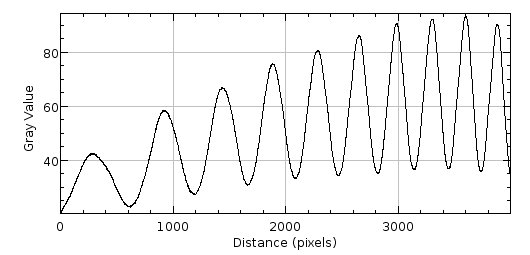
\includegraphics[height=5cm]{pics/Plot_480nm_B=0.jpg}
  \caption{Plot.}
  \label{fig:p5}
\end{figure}
\begin{figure}[h!]
  \centering
  \includegraphics[height=5cm]{pics/Plot_06_480nm_B=0,981_Pol=90°.jpg}
  \caption{Plot.}
  \label{fig:p6}
\end{figure}

\begin{table}[h!]
\parbox{0.48\textwidth}{% 
  \centering
  \sisetup{round-mode = places , round-precision = 0,scientific-notation=fixed, fixed-exponent = 0}
  \begin{tabular}{S} 
    \toprule
    $\text{Position der Intensitätsmaxima} / \symup{px} $\\
    \midrule
      1.090000000000000000e+02\\
      4.680000000000000000e+02\\
      8.310000000000000000e+02\\
      1.186000000000000000e+03\\
      1.536000000000000000e+03\\
      1.883000000000000000e+03\\
      2.217000000000000000e+03\\
      2.542000000000000000e+03\\
      2.868000000000000000e+03\\
      3.185000000000000000e+03\\
      3.494000000000000000e+03\\
      3.803000000000000000e+03\\
    \bottomrule
  \end{tabular}
  \caption{Tabellenunterschrift}
  \label{tab:tab}
}
\parbox{0.48\textwidth}{%
  \centering
  \sisetup{round-mode = places , round-precision = 0,scientific-notation=fixed, fixed-exponent = 0}
  \begin{tabular}{S}
    \toprule
     $\text{Gangunterschied}\; \Delta s / \symup{px} $\\
    \midrule
     6.340000000000000000e+02\\
     5.140000000000000000e+02\\
     4.480000000000000000e+02\\
     4.030000000000000000e+02\\
     3.630000000000000000e+02\\
     3.320000000000000000e+02\\
     3.220000000000000000e+02\\
     2.970000000000000000e+02\\
     2.770000000000000000e+02\\
    \bottomrule
  \end{tabular}
  \caption{Tabellenunterschrift}
  \label{tab:tab}
}
\end{table}

\begin{table}[h!]
  \centering
  \sisetup{round-mode = places , round-precision = 0,scientific-notation=fixed, fixed-exponent = 0}
  \begin{tabular}{S S S}
    \toprule
     \multicolumn{2}{c}{$\text{Postion der Aufspaltungsmaxima} /\symup{px} $} 
     & $\text{Aufspaltung}\; \delta s /\symup{px}  $\\
    \midrule
      3.380000000000000000e+02 & 5.080000000000000000e+02 & 1.700000000000000000e+02\\
      6.920000000000000000e+02 & 8.560000000000000000e+02 & 1.640000000000000000e+02\\
      1.041000000000000000e+03 & 1.207000000000000000e+03 & 1.660000000000000000e+02\\
      1.387000000000000000e+03 & 1.556000000000000000e+03 & 1.690000000000000000e+02\\
      1.737000000000000000e+03 & 1.891000000000000000e+03 & 1.540000000000000000e+02\\
      2.073000000000000000e+03 & 2.225000000000000000e+03 & 1.520000000000000000e+02\\
      2.391000000000000000e+03 & 2.556000000000000000e+03 & 1.650000000000000000e+02\\
      2.722000000000000000e+03 & 2.879000000000000000e+03 & 1.570000000000000000e+02\\
      3.046000000000000000e+03 & 3.190000000000000000e+03 & 1.440000000000000000e+02\\
      3.346000000000000000e+03 & 3.506000000000000000e+03 & 1.600000000000000000e+02\\
      3.670000000000000000e+03 & 3.811000000000000000e+03 & 1.410000000000000000e+02\\
    \bottomrule
  \end{tabular}
  \caption{Tabellenunterschrift}
  \label{tab:tab}
\end{table}


\FloatBarrier







